% =====================================================================
% Expt Fig 4: Varying total data at the base cell d=12, w=768.
% Identifying the data-limited exponent r_P, and asking whether the
% overfit-onset epoch shifts with P.
% =====================================================================


% --- 4.1: val curves across df ---

\begin{figure}[t]
\centering
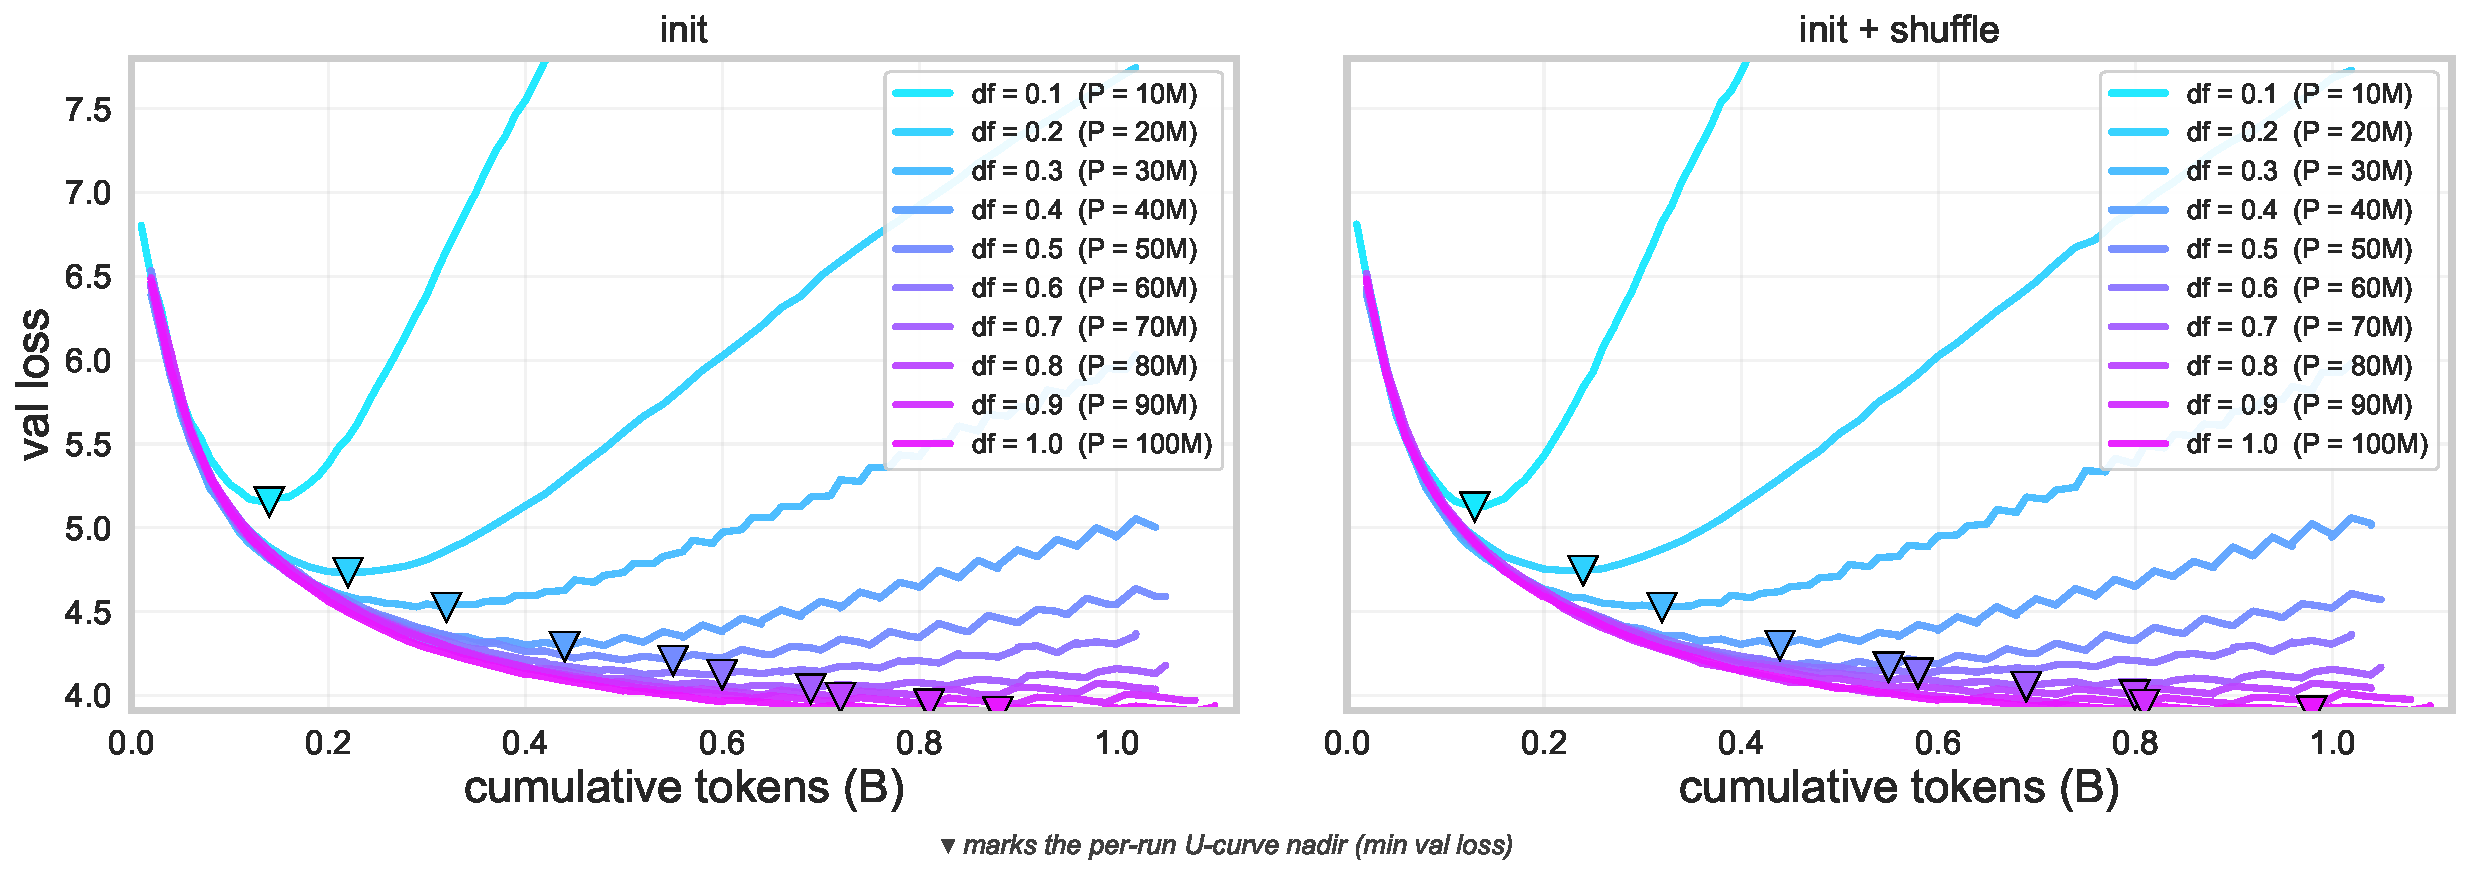
\includegraphics[width=0.99\linewidth]{experiments/figures/04_TBD/expt_fig4_1_val_curves.pdf}
\caption{Validation loss vs cumulative tokens at the base cell ($d{=}12, w{=}768$) for ten unique-data fractions $df \in \{0.1, 0.2, \dots, 1.0\}$ (corresponding to unique tokens $P \in \{10, 20, \dots, 100\}$M of a 100M-token FineWeb subset), shown for both ensembling strategies. Each run trains for the same total budget of $\sim$1B tokens, so larger $df$ corresponds to fewer epochs (101, 51, 34, 26, 21, 17, 15, 13, 12, 11 respectively). $\blacktriangledown$ marks the per-run U-curve nadir.}
\label{fig:datasize_curves}
\end{figure}

\paragraph{Notes on Figure~\ref{fig:datasize_curves}.}
All runs share the same model (base cell), the same total compute, and the same constant LR schedule.
The minimum val loss attained drops monotonically with $P$: $\{5.15, 4.73, 4.53, 4.29, 4.21, 4.12, 4.04, 3.99, 3.95, 3.90\}$ for $df \in \{0.1, 0.2, \dots, 1.0\}$ in the init strategy (init plus shuffle within $0.02$ nat at every $df$) --- a $1.25$-nat range across a $10\times$ range in unique data.
The post-overfit climb is sharply asymmetric: at $df = 0.1$ ($P = 10$M) the val loss climbs back above $7$ nats by $1$B tokens, while at $df \geq 0.7$ the climb is essentially absent within the training budget --- the run is effectively single-pass and never enters the variance-dominated regime.
Both strategies behave nearly identically at the base cell --- the strategy difference that dominated Expts 2 and 3 (where ensembling was the main compute axis) is not visible in the single-model ($E = 1$) view.


% --- 4.2: r_P fit + onset ---

\begin{figure}[t]
\centering
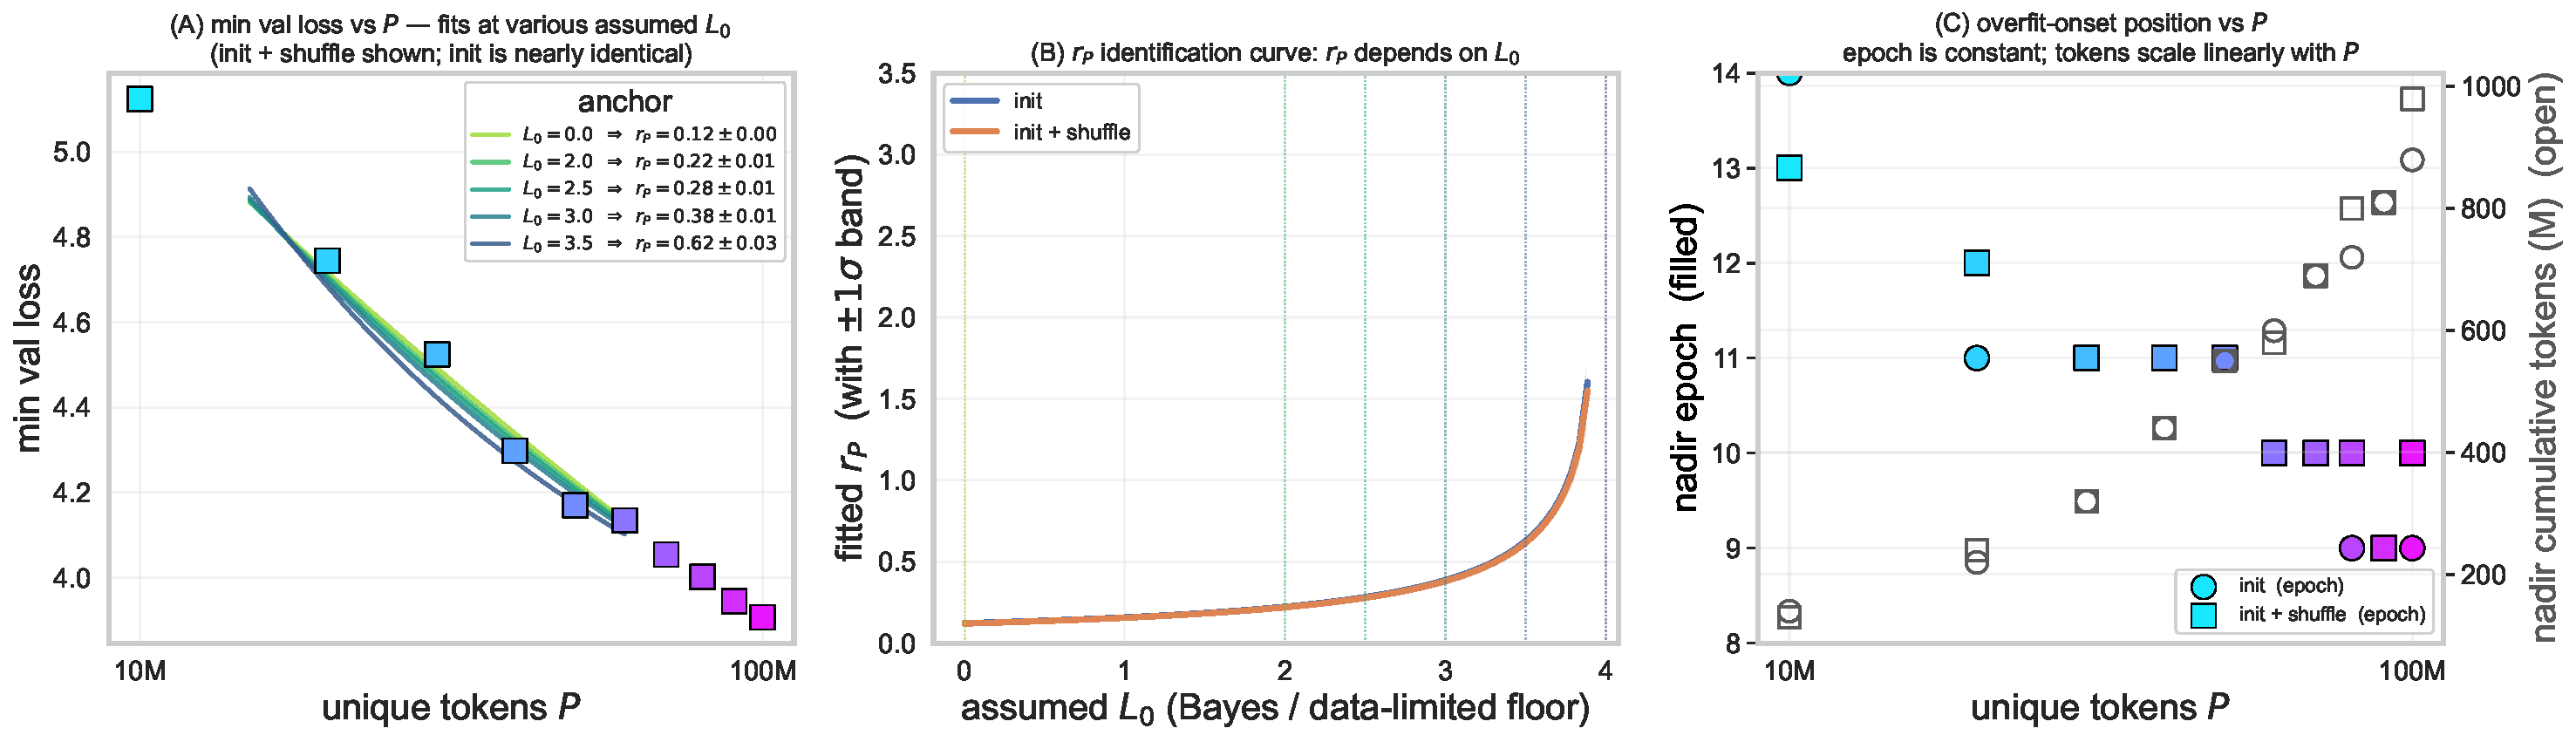
\includegraphics[width=0.99\linewidth]{experiments/figures/04_TBD/expt_fig4_2_rP_fit.pdf}
\caption{Fitting the data-limited exponent $r_P$ from the per-run U-curve nadirs, and analysis of the overfit-onset position. (A) Per-run min val loss vs $P$, overlaid with fits at five different assumed values of $L_0$ (the data-limited / Bayes-error floor); only init plus shuffle is shown for clarity (init is nearly identical). (B) The corresponding identification curve: fitted $r_P$ as a function of assumed $L_0$, with $\pm 1\sigma$ uncertainty band, for both strategies. (C) Per-run nadir position vs $P$: the nadir epoch (filled markers, left axis) and the nadir cumulative tokens (open markers, right axis).}
\label{fig:rP_fit}
\end{figure}

\paragraph{Notes on Figure~\ref{fig:rP_fit}.}
Premise: at the per-run U-curve nadir, the variance-buildup and bias-dynamics terms in the proposed law are at their minima, so $\min_t L(t)$ should approximately equal $c_P P^{-r_P} + L_{0,\mathrm{eff}}$, where $L_{0,\mathrm{eff}}$ absorbs the (constant) parameter-bias contribution and the residual bias dynamics at the nadir.
With $10$ $P$ values per strategy, the $3$-parameter fit $(c_P, r_P, L_0)$ is well-conditioned (7 dof) and the unconstrained NLLS converges to $r_P = 0.19 \pm 0.06$ with $L_0 = 1.58 \pm 0.86$ for init, and $r_P = 0.17 \pm 0.08$ with $L_0 = 1.22 \pm 1.47$ for init plus shuffle, with per-observation residual $\hat\sigma \approx 0.024$--$0.031$.
The data alone prefer a low $L_0$ ($\approx 1.5$ nat), which is below the typical Bayes-error proxy for FineWeb val on a 1.8B-parameter GPT.
Panel (B) traces the $L_0$-dependence: $r_P$ grows from $\approx 0.12$ at $L_0 = 0$ to $\approx 0.62$ at $L_0 = 3.5$, with $L_0 = 4.0$ no longer feasible because the smallest $\min_t L = 3.91$ falls below it.
At physically plausible Bayes-error anchors $L_0 \in \{2.5, 3.0\}$ nats, $r_P \in \{0.28, 0.38\}$ for both strategies, broadly compatible with the Chinchilla-style data-scaling exponent.

\paragraph{Choice of headline value for the joint fit.}
The data-driven unconstrained fit returns $r_P \approx 0.18$ with $L_0 \approx 1.5$, while a Chinchilla-style $L_0 \in [2.5, 3.0]$ prior pushes $r_P$ to $0.28$--$0.38$.
The 2$\sigma$ wide $L_0$ uncertainty leaves us unable to distinguish the two regimes from $\min_t L$ alone --- the difference shows up only at the smallest-$P$ tail of the curve, where the bias-dynamics term contribution to $\min_t L$ is most uncertain.
For the joint scaling-law fit that combines all four experiments, we therefore propagate this uncertainty by reporting $r_P$ at three anchors $L_0 \in \{0, 2.5, 3.0\}$ rather than picking a single point estimate; the qualitative conclusion that $r_P$ is positive (data helps) is robust across the entire $L_0$ range, but the rate is conditional on the $L_0$ choice.

\paragraph{Overfit-onset weakly tracks $P$.}
Panel (C) shows that the nadir epoch is a slowly decreasing function of $P$: it sits at epoch $\approx 13$ at $P = 10$M, drops to $\approx 11$ at $P = 30$--$50$M, and is at $\approx 9$--$10$ at $P \geq 60$M.
Two effects are entangled in this plot.
For small $df \leq 0.5$, where the U-curve is well-developed within the $1$B-token budget, the nadir is a meaningful overfit-onset measurement and the small drift toward earlier epochs likely reflects faster onset of the variance-dominated regime when there is less unique data per epoch.
For large $df \geq 0.7$, the $1$B-token budget is barely longer than one full pass, the U-curve climb is not visible (Figure~\ref{fig:datasize_curves}), and the ``nadir epoch'' is essentially the last epoch where loss is still descending --- not a true overfit-onset.
Compared to the cumulative-token nadir, which scales near-linearly with $P$ (open markers go from $130$M to $980$M as $P$ goes from $10$M to $100$M), the epoch nadir varies much less, consistent with the conjecture that the variance-buildup term $(s/T)^\delta$ uses $s/T$ as an epoch-counter argument that is not strongly $P$-dependent.


% --- body ---

The proposed scaling law splits the loss into a parameter-driven bias floor $(N^2 L)^{-r_{\mathrm{param}}}$, a data-limited floor $P^{-r_P}$, a bias-dynamics term $s^{-r_t}$, the variance-buildup term $E^{-\delta_E} N^{\delta_N} L^{\delta_L} (s/T)^\delta$, and an irreducible $\mathcal{L}_0$.
Expts 2 and 3 held $P$ fixed and identified $\delta_E$ (Expt 2) and the structural exponents $\delta_N, \delta_L$ (Expt 3); Expt 4 turns the $P$ knob to recover $r_P$.
Two findings emerge.

First, the data-limited exponent $r_P$ is real and clearly positive --- $\min_t L$ drops from $5.15$ at $P = 10$M to $3.91$ at $P = 100$M, a factor-of-$10$ extension of unique data buys roughly $1.25$ nats of val loss --- but its precise value depends on the assumed Bayes-error floor.
The unconstrained fit prefers $r_P \approx 0.18$ with $L_0 \approx 1.5$; a Chinchilla-style prior $L_0 \in [2.5, 3.0]$ gives $r_P \in [0.28, 0.38]$.
The $(r_P, L_0)$ pair traces a one-dimensional ridge along which any combination $r_P \in [0.12, 0.62]$ is consistent with the data depending on $L_0$ (Panel~B).
Resolving this in future work likely requires either anchoring $L_0$ from a long-training extrapolation past the U-curve climb at fixed $P$, or extending the $df$ sweep with more FineWeb beyond the current 100M-token universe to gain leverage on the high-$P$ asymptote.

Second, the overfit-onset is approximately epoch-driven at the base cell.
Across a $10\times$ change in $P$, the nadir epoch drifts only from $13$ down to $9$, while the nadir cumulative-token count rises by an order of magnitude from $130$M to $\approx 1$B.
This is consistent with the variance-buildup term in the proposed law having the form $(s/T)^\delta$, where $s/T$ is the epoch counter --- once a run enters the variance-dominated regime, it is the number of repeats (epochs) that determines onset, not the unique-token volume.
The mild remaining $P$-dependence of the nadir epoch is well within what would be expected from the bias-dynamics term $s^{-r_t}$ shifting the nadir slightly even when the variance-buildup term is purely epoch-driven --- the bias term reaches its asymptote later in tokens for runs with larger $P$, slightly delaying the crossover with the rising variance term.

Reading Expts 1--4 together, the combined picture is that the four contributions to the loss can be measured along the four axes of variation we sweep: bias dynamics in $s$ (any of the four experiments), $\delta_E$ in $E$ (Expt 2 with the widest ensemble grid), $\delta_N$ and $\delta_L$ in $(N, L)$ (Expt 3 with the $4 \times 4$ grid), and $r_P$ in $P$ (Expt 4, modulo the $L_0$-degeneracy).
The conjectured $\delta = 1/2$ for the epoch dependence of variance buildup is the only piece our data strongly contradicts (Expt 3 prefers $\delta \gtrsim 2$); the other three structural exponents are either pinned ($\delta_E$, $\delta_N$, $\delta_L$, $r_t$) or pinned-modulo-prior ($r_P$).
A clean joint fit on all four experiments is the natural next step, and is enabled by the combined data export tables associated with this paper.
